% Template for PLoS
% Version 3.4 January 2017
%
% % % % % % % % % % % % % % % % % % % % % %
%
% -- IMPORTANT NOTE
%
% This template contains comments intended 
% to minimize problems and delays during our production 
% process. Please follow the template instructions
% whenever possible.
%
% % % % % % % % % % % % % % % % % % % % % % % 
%
% Once your paper is accepted for publication, 
% PLEASE REMOVE ALL TRACKED CHANGES in this file 
% and leave only the final text of your manuscript. 
% PLOS recommends the use of latexdiff to track changes during review, as this will help to maintain a clean tex file.
% Visit https://www.ctan.org/pkg/latexdiff?lang=en for info or contact us at latex@plos.org.
%
%
% There are no restrictions on package use within the LaTeX files except that 
% no packages listed in the template may be deleted.
%
% Please do not include colors or graphics in the text.
%
% The manuscript LaTeX source should be contained within a single file (do not use \input, \externaldocument, or similar commands).
%
% % % % % % % % % % % % % % % % % % % % % % %
%
% -- FIGURES AND TABLES
%
% Please include tables/figure captions directly after the paragraph where they are first cited in the text.
%
% DO NOT INCLUDE GRAPHICS IN YOUR MANUSCRIPT 
% - Figures should be uploaded separately from your manuscript file. 
% - Figures generated using LaTeX should be extracted and removed from the PDF before submission. 
% - Figures containing multiple panels/subfigures must be combined into one image file before submission.
% For figure citations, please use "Fig" instead of "Figure".
% See http://journals.plos.org/plosone/s/figures for PLOS figure guidelines.
%
% Tables should be cell-based and may not contain:
% - spacing/line breaks within cells to alter layout or alignment
% - do not nest tabular environments (no tabular environments within tabular environments)
% - no graphics or colored text (cell background color/shading OK)
% See http://journals.plos.org/plosone/s/tables for table guidelines.
%
% For tables that exceed the width of the text column, use the adjustwidth environment as illustrated in the example table in text below.
%
% % % % % % % % % % % % % % % % % % % % % % % %
%
% -- EQUATIONS, MATH SYMBOLS, SUBSCRIPTS, AND SUPERSCRIPTS
%
% IMPORTANT
% Below are a few tips to help format your equations and other special characters according to our specifications. For more tips to help reduce the possibility of formatting errors during conversion, please see our LaTeX guidelines at http://journals.plos.org/plosone/s/latex
%
% For inline equations, please be sure to include all portions of an equation in the math environment.  For example, x$^2$ is incorrect; this should be formatted as $x^2$ (or $\mathrm{x}^2$ if the romanized font is desired).
%
% Do not include text that is not math in the math environment. For example, CO2 should be written as CO\textsubscript{2} instead of CO$_2$.
%
% Please add line breaks to long display equations when possible in order to fit size of the column. 
%
% For inline equations, please do not include punctuation (commas, etc) within the math environment unless this is part of the equation.
%
% When adding superscript or subscripts outside of brackets/braces, please group using {}.  For example, change "[U(D,E,\gamma)]^2" to "{[U(D,E,\gamma)]}^2". 
%
% Do not use \cal for caligraphic font.  Instead, use \mathcal{}
%
% % % % % % % % % % % % % % % % % % % % % % % % 
%
% Please contact latex@plos.org with any questions.
%
% % % % % % % % % % % % % % % % % % % % % % % %

\documentclass[10pt,letterpaper]{article}
\usepackage[top=0.85in,left=2.75in,footskip=0.75in]{geometry}

% amsmath and amssymb packages, useful for mathematical formulas and symbols
\usepackage{amsmath,amssymb}

% Use adjustwidth environment to exceed column width (see example table in text)
\usepackage{changepage}

% Use Unicode characters when possible
\usepackage[utf8x]{inputenc}

% textcomp package and marvosym package for additional characters
\usepackage{textcomp,marvosym}

% cite package, to clean up citations in the main text. Do not remove.
\usepackage{cite}

% Use nameref to cite supporting information files (see Supporting Information section for more info)
\usepackage{nameref,hyperref}

% line numbers
\usepackage[right]{lineno}

% ligatures disabled
\usepackage{microtype}
\DisableLigatures[f]{encoding = *, family = * }

% color can be used to apply background shading to table cells only
\usepackage[table]{xcolor}

% array package and thick rules for tables
\usepackage{array}

\usepackage{bm}


% create "+" rule type for thick vertical lines
\newcolumntype{+}{!{\vrule width 2pt}}

% create \thickcline for thick horizontal lines of variable length
\newlength\savedwidth
\newcommand\thickcline[1]{%
  \noalign{\global\savedwidth\arrayrulewidth\global\arrayrulewidth 2pt}%
  \cline{#1}%
  \noalign{\vskip\arrayrulewidth}%
  \noalign{\global\arrayrulewidth\savedwidth}%
}

% \thickhline command for thick horizontal lines that span the table
\newcommand\thickhline{\noalign{\global\savedwidth\arrayrulewidth\global\arrayrulewidth 2pt}%
\hline
\noalign{\global\arrayrulewidth\savedwidth}}


% Remove comment for double spacing
%\usepackage{setspace} 
%\doublespacing

% Text layout
\raggedright
\setlength{\parindent}{0.5cm}
\textwidth 5.25in 
\textheight 8.75in

% Bold the 'Figure #' in the caption and separate it from the title/caption with a period
% Captions will be left justified
\usepackage[aboveskip=1pt,labelfont=bf,labelsep=period,justification=raggedright,singlelinecheck=off]{caption}
\renewcommand{\figurename}{Fig}

% Use the PLoS provided BiBTeX style
\bibliographystyle{plos2015}

% Remove brackets from numbering in List of References
\makeatletter
\renewcommand{\@biblabel}[1]{\quad#1.}
\makeatother

% Leave date blank
\date{}

% Header and Footer with logo
\usepackage{lastpage,fancyhdr,graphicx}
\usepackage{epstopdf}
\pagestyle{myheadings}
\pagestyle{fancy}
\fancyhf{}
\setlength{\headheight}{27.023pt}
\lhead{
\includegraphics[width=2.0in]{PLOS-submission.eps}}
\rfoot{\thepage/\pageref{LastPage}}
\renewcommand{\footrule}{\hrule height 2pt \vspace{2mm}}
\fancyheadoffset[L]{2.25in}
\fancyfootoffset[L]{2.25in}
\lfoot{\sf PLOS}

%% Include all macros below

\newcommand{\lorem}{{\bf LOREM}}
\newcommand{\ipsum}{{\bf IPSUM}}

\def\EMG/{\textsc{emg}}
\def\EEG/{\textsc{eeg}}
\def\REM/{\textsc{rem}}
\def\NREM/{\textsc{nrem}}
\def\WK/{\textsc{wk}}
\def\WKL/{\textsc{wkl}}
\def\WKB/{\textsc{wkb}}
\def\SWC/{\textsc{swc}}
\def\BD/{\textsc{bd}}
\def\TP/{\textsc{tp}}
\def\KM/{\textsc{km}}
\def\LD/{\textsc{ld}}
\def\EEG/{\textsc{eeg}}
\def\EMG/{\textsc{emg}}




\newcommand{\pp}[2]{\bm{p_{#1 \rightarrow #2}}}
\newcommand{\pms}[1]{\bm{p_{#1}}}

%% END MACROS SECTION


\begin{document}
\vspace*{0.2in}

% Title must be 250 characters or less.
\begin{flushleft}
{\Large
\textbf\newline{ A four-state Markov model of  sleep-wakefulness dynamics along light/dark cycle in mice} % Please use "sentence case" for title and headings (capitalize only the first word in a title (or heading), the first word in a subtitle (or subheading), and any proper nouns).
}
\newline
% Insert author names, affiliations and corresponding author email (do not include titles, positions, or degrees).
\\
Lonel Perez-Atencio \textsuperscript{2},
Nicolas Garcia-Aracil\textsuperscript{1},
Eduardo Fernandez\textsuperscript{1},
Luis C. Barrio\textsuperscript{2},
Juan A. Barios\textsuperscript{1*}
\\
\bigskip
\textbf{1} Biomedical Neuroengineering research group (nBio), Systems Engineering and Automation Department of Miguel Hernandez University, Avda. de la Universidad s/n, 03202 Elche, Spain
\\
\textbf{2} Unit of Experimental Neurology, “Ram\'on y Cajal” Hospital-IRYCIS, Carretera de Colmenar km 9, 28034 Madrid, Spain
\\
\bigskip

* Correspondence: jbarios@umh.es

\end{flushleft}
% Please keep the abstract below 300 words
\section*{Abstract}
Behavioral states alternate between wakefulness (\WK/), rapid eye movement (\REM/) and non-\REM/ (\NREM/) sleep  at time scale of hours (i.e., circadian and ultradian rhythms) and from several tens of minutes to seconds (i.e., brief awakenings during sleep). Using statistical analysis of bout duration,   Markov chains of sleep-\WK/ dynamics and quantitative EEG  analysis, we evaluated  the influence of circadian light/dark (\LD/) changes on brain function along the sleep-\WK/ cycle. Bout duration (\BD/) histograms and Kaplan-Meier (\KM/) survival curves of \WK/  showed a bimodal statistical distribution, suggesting that  two types of \WK/ do exist:  brief-\WK/ (\WKB/) and long-\WK/ (\WKL/). Circadian light changes modulated specifically \WKL/ bouts, increasing its duration during active/dark period. In contrast, \NREM/ and \REM/ \BD/ histograms and \KM/ curves did not change significantly along \LD/ cycle.  Hippocampal \EEG/ of both types of \WK/ were different: in \WKL/, we found i)\,higher  fast gamma and theta \EEG/ power and increased \EMG/ tone; ii)\,faster theta peak frequency. After fitting a four-states Markov chain to mice hypnograms, circadian modulation of \TP/ was found:  in dark/active period,  state-maintenance probability of \WKL/ increased, and probability  of \WKL/ to \NREM/ transition  decreased; the opposite was found in light period. In conclusion, we propose an extended Markov model of sleep using four stages (\WKL/,  \NREM/, \REM/, \WKB/) as a fully adequate model accounting for both the circadian and ultradian modulation of sleep-wake dynamics based on the differential regulation of long-\WK/  (high gamma/theta) epochs  during dark and light phases.


\linenumbers

\section{Introduction}
The sleep-wake cycle (\SWC/)  is a dynamic phenomenon, resulting from complex interactions between the activity of neuronal populations in many brain structures, including the basal forebrain, hypothalamus and brainstem. Appropriate control of this brain activity permits behavioural state transitions between \WK/, \REM/ and \NREM/ sleep   \cite{Scammell2017,Ferri2016}. Cycling between sleep and \WK/ is regulated at time scales of seconds to several tens of minutes by the intrinsic activity of sleep-wake neuronal networks and of hours under control of circadian and ultradian rhythms \cite{Borbely1982,Phillips2007}. Main circadian oscillator regulating the brain arousal system is located in the suprachiasmatic nucleus \cite{Aston-Jones2001,fleshner2011circadian}. The cyclic sequence of \NREM/ and \REM/ sleep, or the so-called ultradian rhythm, is a highly characteristic feature of sleep.  Molecules such as hypocretins (Hcrt), also called orexins,  help to stabilize state changes. Loss of Hcrt in mice with a knockout of this gene leads to fragmentation of sleep, i.e., shorter wake and sleep bouts \cite{chemelli1999narcolepsy}. Thus, specific molecules may control not only the amount of sleep and wakefulness but also the maintenance of sleep and hence the bout length of different states.

Wakefulness changes in the \EEG/ are useful  to distinguish it from deeper sleep stages, so that modifications of electrical activity are considered as  biomarkers for predicting changes in the capability of animals to represent and respond to stimuli. Activity of Hcrt neurons is linked to heightened attentional states\cite{sasaki2011pharmacogenetic},  and also to EEG frequencies in the gamma range ($>30$\,Hz), a main characteristic of \WK/ states \cite{Lee2005,alexandre2013control,mcginley2015waking}.   Rodent waking is often divided into quiet and active \WK/ based on whether the animal is still or exhibits exploratory movements. Transitions from quiet to active wake correlate with increased theta and gamma power,  although detailed studies of activity changes in different modalities of \WK/ and its relation with wake duration are lacking \cite{vassalli2017hypocretin}. 
 

 Existence of short and long bouts of sleep and wakefulness is a  basic feature of sleep/wake control  found in mammals  \cite{Lo2004}.  Different duration of bouts of sleep and wake have been analyzed using survival curve analysis.  This technique measures the probability that a given bout will survive long enough to reach a given duration, plotting the percentage of a state as a function of different bout length. For wakefulness a log–log plot leads to a linear description, i.e., a power-law distribution, while for sleep a semi-log plot, i.e., an exponential distribution, is best \cite{Lo2004,Behn2007,behn2008delayed,Simasko2009,McShane2010}. The resulting survival curves can be statistically analyzed to evaluate the sleep structure and underlying mechanisms, e.g in rats \cite{stephenson2013statistical}, mice \cite{McShane2010} or humans \cite{klerman2013survival}.

Although presence of  circadian and ultradian rhythms along the  \SWC/ is a clear indication of the existence of time-dependent variations in sleep architecture, transitions between sleep-wake states show a high degree of apparently random variability, suggesting that  statistical tools should also be a useful way for studying sleep dynamics. Markov chains represent a class of stochastic processes of great interest for a wide spectrum of practical applications; in particular, discrete time Markov chains permit to model the transition probabilities between discrete states \cite{zung1966computer,Kemp1986,Bremaud1999,Spedicato2015}, allowing to model the dynamics of \SWC/ in mammals. Markov chains have also been used for studying physiology of human sleep \cite{Kemp1986}, and some clinical applications of these methods have also been reported \cite{Kim2009,Ferri2016,Bianchi2012,wei2017sleep}. For example, Markov chains have been used for studying  polisomnographies  of patients with narcolepsy, where a deficit of Hcrt produces a sleep with normal amounts of sleep and wake, but very brief states with increased transitions between them \cite{Ferri2016}, findings also present in  the knockout-Hcrt mouse model  \cite{Mochizuki2004}. Given the stochastic nature of state transitions along the \SWC/ under normal and pathological conditions, \SWC/ are well suited to be modeled by discrete time Markov chains. Markov analysis provides accurate information of the probability of staying in one state (i.e., state stability, closely related to state duration), and of the transition probabilities from and to that state, that cannot be obtained by other existing methods. 



The current study was designed to describe the functional  differences between Brief and Long \WK/ and  to study the  modulation induced by circadian dark/light changes over the sleep-wake pattern. Our data indicate that a better description of the sleep-wake architecture along \LD/ cycle results extending the usual three-state model (\WK/,  \NREM/, \REM/) to  a four-state (\WKL/,  \NREM/, \REM/, \WKB/) Markov model.


\section{Material and Methods}

\subsection{Animals}
Male wild-type mouse (C57Bl/6) of three-month age were used in this study (N= 10). All experimental procedures were approved by Institutional Animal Care and Use Committee of Ram\'on y Cajal Hospital (Madrid, Spain) in accordance with Spanish (R.D. 1201/2005) and the Council Directive
2010/63EU of the European Parliament and the Council of 22 September
2010 on the protection of animals used for scientific purposes. 


\subsection{Surgery and EEG/EMG recordings}
Animals were implanted under anesthesia with 1.5\% isoflurane in 100\% oxygen an electrode of nickel-chromium (140 microns) in prefrontal cortex (1.5 mm rostral, 1.5 mm lateral and 1 mm ventral to bregma), a second electrode in the CA1 region of hippocampus (-2.4 mm rostral, 1.5 mm lateral, 1.5 mm ventral), two stainless steel screws in the pre-frontal region, for ground and indifferent references, and a silver plate in the muscles of the neck for \EMG/ recording. Recovery took place in an isolated chamber under 12:12h \LD/ regime. Nine days after surgery, mice were transferred to a circular  cage and the implanted cap fixed to a rotating anti-gravitational connector allowing free movements; \LD/ was not changed. After period of habituation of 72 h in the sound attenuated chamber (12-h light/12-h dark cycle; constant temperature 22-24 ºC; light onset at 08:00 hours; \emph{ad libitum} access to food and water; 10 Watt  energy saving lamp, approximately 30 lux), 24 h of uninterrupted recording were acquired.  \EEG/ of the cortex, hippocampus and \EMG/ signals were filtered from 0.5 Hz to 500 Hz, amplified (x5000-10,000) (Cyberamp 380, Axon Instruments) and digitized at 1 kHz (Axon CNS Digidata 1440).

\subsection{Sleep-wake staging}

Sleep scoring was accomplished using an offline automated sleep scoring system, based on  custom scripts (\textsc{matlab} 2008, Mathworks, \textsc{usa}). For automated staging,  z-score of rms of band filtered  \EEG//\EMG/ signals was calculated from  cortex; $\delta_{cx}$ (1-4 Hz),  $\sigma_{cx}$ (10-15 Hz), $\beta_{cx}$ (15-25 Hz); hippocampus, $\theta_{hc}$  (7-10 Hz),  $\gamma_{hc}^{1}$ (25-55 Hz); $\gamma_{hc}^{2} $ (55-125 Hz); and \EMG/  (55-90 Hz).  $\theta_{hc}/ \delta_{cx}$ and $\beta_{cx}/ \gamma_{hc}^{1}$ indexes were calculated.   Initially, epochs with low  $\beta_{cx}/ \gamma_{hc}^{1}$,  high $\theta_{hc}/ \delta_{cx}$ and high \EMG/ are assigned to \WK/, epochs with low $\theta_{hc}/ \delta_{cx}$,  high $\beta_{cx}/ \gamma_{hc}^{1}$ and low \EMG/ to \NREM/, and epochs with high $\theta_{hc}/ \delta_{cx}$  and low \textsc{\EMG/} to \REM/, using a fixed  threshold, and non-assigned epochs were classified in a first pass of \textsc{matlab}  K-$means$ algorithm. Then, thresholds were recalculated and  a second pass of the algorithm determined the definitive staging.  This analysis classified every 5 seconds epochs in \WK/, \NREM/ and \REM/ states. Automated scoring was examined and visually corrected  by two expert scorers. For helping in the analysis, quantified indexes of \EEG//\EMG/ recordings were  used by the scorers as an aid in ambiguous scoring epochs. 

In order to evaluate  staging, spectral analysis of staged epochs was performed. \NREM/ epochs shown a predominance of low frequency (1-4 Hz). In cortex and hippocampus, \REM/ epochs had a predominance of hippocampal theta (7-10 Hz) activity and a desynchronization between cortex and hippocampus that is evidenced by the distinctive behavior of the spectral curves between the regions of the brain previously described. After staging, the corresponding polysomnograms are constructed for each mouse recording, and mean duration and total amount of each state for 12 h of dark and light periods were calculated. For the visual analysis of the signals we used the software \textsc{spike 2 (v 6.18, ced, uk)}.



\subsection{Data analysis}
 
After staging, analysis of recordings was performed using two complementary approaches: (1) for each state, bout durations (measured to the nearest 5-sec epoch) were evaluated using survival curves. (2) state-to-state transition probabilities were quantified using a Markov analysis.


\subsubsection{Survival curves:} Bout durations (min) of each recording were processed by Kaplan-Meier survival curve analysis using 5-sec (i.e. single epoch) time bins: $S_ {(ti)} = S_{ (ti-1)}*((r_i-d_i)/r_i)$ where $S_ {(ti)}$ is the proportion of the original number of bouts surviving at the end of time bin $ti$, $S_{ (ti-1)}$ is the proportion of the original number of bouts remaining one time bin before $ti$, $r_i$ is the number of bouts remaining at the start of time bin $ti$, and $d_i$ is the number of bouts that terminate during time bin $ti$.  Initially, the analysis was performed without reference to time-dependent factors (i.e., in each animal, all data were pooled; “24-h pooled”). To evaluate circadian modulation, light and dark epochs were then examined separately.
 
\subsubsection{Markov chains:} A discrete time Markov chain is a sequence of random variables characterized by the Markov property, by which the state S at any time $t+1$ depends on the state at time $t$ but not on previous history. State transition probabilities describe the probability of going from stage i to stage j in a discrete time step (n) of 5 seconds: $P_{ij}=P_r(X_n=j|X_o=i)$.  The transition probabilities of Markov chains between the 4 \WK/-sleep states (long \WK/, brief \WK/,  \NREM/ and \REM/)  were arranged in a matrix with the form 
\[
\begin{bmatrix}
P_{\WKL/ \rightarrow \WKL/} & P_{\WKL/ \rightarrow \WKB/} & P_{\WKL/ \rightarrow \NREM/} & P_{\WKL/ \rightarrow\REM/} \\
P_{\WKB/ \rightarrow \WKL/} & P_{\WKB/ \rightarrow \WKB/} & P_{\WKB/ \rightarrow \NREM/} & P_{\WKB/ \rightarrow\REM/} \\
P_{\NREM/ \rightarrow \WKL/} & P_{\NREM/ \rightarrow \WKB/} & P_{\NREM/ \rightarrow \NREM/} & P_{\NREM/ \rightarrow\REM/} \\
P_{\REM/ \rightarrow \WKL/} & P_{\REM/ \rightarrow \WKB/} & P_{\REM/ \rightarrow \NREM/} & P_{\REM/ \rightarrow\REM/} 
\end{bmatrix}
.\]  
where each element of position $(i,j)$ represents the transition probability $P_{i\rightarrow j}$: e.g, probability of transition from \NREM/ state to \REM/ state is denoted as $P_{\NREM/\rightarrow \REM/}$. State maintenance probabilities, ($p_{ii}$) that describe the probability of remaining in one state, are denoted as $P_{\WKL/}$, $P_{\WKB//}$, $P_{\NREM/}$, $P_{\REM/}$. Markov chains have been already validated as a  model for sleep dynamics in mouse and rat \cite{stephenson2013statistical}, so we did not perform specific tests to validate prior Markov analysis assumptions. Markov analysis was performed using the markovchain package (R environment, ver. 0.6.5.1) \cite{Spedicato2015}. 

\subsubsection{EEG Power Spectral Analysis}.

EEG signals were subjected to discrete Fourier transform to determine EEG power density spectra (0 to 120 Hz) for 5-s windows (Hamming function) with 0.20-Hz frequency resolution. Mean EEG spectral profiles for each behavioral state and time interval were calculated using artifact-free 5-s epochs.  Time-course of activity in different bands  was  calculated by averaging power density in the corresponding frequency bins. To account for interindividual differences in absolute EEG power, power density in each frequency bin and for each state was expressed as a z-score of  each individual mouse.

\subsection{Statistical analysis}

Data were presented as mean value or percentage of total value$\pm \textsc{se}$. Differences between the groups were evaluated using the Student's t-test, Mann-Whitney test, and Bonfferoni test (Anova), depending on the compliance with the normality hypothesis of the data using  Sigmaplot (San Rafael, Hearne Scientific Software, 2006) and R statistical software \cite{R2008}. 

\section{Results}

Quantitative analysis of state durations showed that total amount of \WK/ epochs increased significantly in dark phase in comparison with light phase, while \NREM/ and \REM/ decreased ($p < 0.05$) (Fig. 2A). Histograms of bout-duration \BD/ for each state were also obtained for dark and light phases (Fig. 2B). Histogram of \WK/  \BD/s showed in both dark and light periods a bimodal distribution corresponding to epochs of brief and long \WK/  (\WKB/  and \WKL/). Interestingly, circadian modulation only affected to \WKL/, shifting its density peak toward longer lasting \WK/ during dark phase ($p < 0.05$), in contrast of \WKB/ \BD/  distribution that did not vary between dark and light. \NREM/- and \REM/-\BD/ distributions approximated respectively to a bimodal and unimodal distributions but neither changed significantly during the phases of dark and light. Accordingly, the survival curve of \WK/ exhibited a biexponential distribution, while \REM/ and \NREM/ survival curves were monoexponential (Fig. 2C). However, only the cumulative distribution corresponding to the longer \WK/  durations of approximately 150 seconds enhanced during for during dark period of circadian rhythm. Thus, data clearly indicate that two types of \WK/ can be segregated by its bout duration: long wakes ($> 150s$) and brief wakes ($< 150s$) and that only the long \WK/ are under control of circadian rhythmicity. Consequently, the dynamics of sleep-wake cycling were analyzed by applying a four-state (\WKL/, \WKB/, \NREM/ and \REM/) Markov model. 

After finding a time threshold able to discriminate between \WKB/ and \WKL/, we tried to evaluate if spectral differences existed between them. In figure ~\ref{fig_eeg} (A), spectral characteristics of both \WK/ substates are shown.  Long-\WK/ epochs had  higher fast gamma power in hippocampus (CA1 region), higher hippocampal theta \EEG/ power and increased \EMG/ tone vs Brief-\WK/. In \WKL/ epochs,  a clear theta frequency peak  of 8 Hz appears  in hippocampus of waking mice (theta rhythm type I, usually associated to locomotion states, marked as ``b'' peak in the figure). Same peak, with reduced power and slower peak frequency (6 Hz) was found in \WKB/ epochs (theta rhythm type II, usually associated to alert immobility) \cite{gangadharan2016medial}. For completeness, we included in the figure the spectral density of \NREM/ and \REM/ epochs, where the expected increase of slow and beta power with gamma power reduction in \NREM/ epochs and the increase of hippocampal theta power in \REM/ epochs can be noticed. EMG tone was also reduced in \WKB/ vs  \WKL/ (figure ~\ref{fig_eeg} (B). 

%In figure ~\ref{fig_eeg} (C), the time course of fast gamma power (60-100 Hz) was evaluated in function of \WK/ duration. Unexpectedly,  we found that it slowly increased from \WK/ onset, with an exponential  time course of several minutes. Differences in amplitude appear clearly, where shorter \WK/ bouts have reduced fast gamma power. 

 
Transition probabilities matrix derived from Markov analysis revealed high probabilities for staying in one state and much lower probabilities of transition between different states (Table 1 and Fig. 3). The order of state maintenance probabilities, which correlated with the corresponding values of bout-duration, was $P_{\WKL/}>P_{\NREM/}>P_{\REM/}>P_{\WKB/},$ with statistically significant differences between all states ($p < 0.001$). State transitions between all behavioral states were theoretically possible with the exception of $ \pp{\WKB/ }{\NREM/} $, by definition of states; the sequence of transition probabilities (i.e., the rate) was as followed: $ \pp{\WKB/ }{\NREM/} \gg \pp{\REM/}{\NREM/} \gg \pp{\WKL/}{ \NREM/} \gg \pp{\NREM/}{\WKL/} \approx \pp{\REM/}{\WKL/} \approx \pp{\REM/}{ \WKB/} \gg \pp{\NREM/}{\WKB/} \approx \pp{\WKL/}{\REM/} \gg \pp{\WKB/}{\REM/} $, revealing that there are important differences in the transitions probability depending on the involved states and its direction. Transitions from \WKB/ and rem to \NREM/ were the most frequent and statistically different each other and with the rest of state transitions ($p < 0.001$), while transitions of $ \pp{\NREM/ }{\WKL/} $, $ \pp{\REM/ }{\WKL/} $, and $ \pp{\REM/ }{\WKB/} $, were more frequent than the transitions of $ \pp{\NREM/ }{\WKB/} $, $ \pp{\WKL/ }{\REM/} $, and $ \pp{\WKB/}{\REM/} $, ($p < 0.05$). Regarding to circadian modulation, only the stability of \WKL/ state varied significantly with circadian rhythm ($p < 0.01$), increasing and decreasing respectively in dark and light phase, and only the probability of state transitions from \WKL/ to \NREM/ decreased significantly in the dark phase in comparison with light period ($p < 0.05$), while $ \pp{\WKL/}{\NREM/} $, was higher than $ \pp{\NREM/ }{\WKL/} $ during the light period ($p < 0.01$) (Fig. 3).


\section{Discussion}

The main findings of this report are that functional differences between long-\WK/ and brief-\WK/ and circadian \LD/ changes modulation of sleep-wake transitions justify a new model of sleep-wake dynamics based in 4 states: long \WK/, brief \WK/, \NREM/ and \REM/ sleep. 

Normal sleep is characterized by the cyclic alternance of \NREM/ and \REM/ sleep (i.e., the so called ultradian \NREM/-\REM/ rhythm). In monophasic sleep, as in humans,  after a first  \NREM/-\REM/ period, two to seven ultradian cycles follow until waking up.  In polyphasic species, such as rodents,  sleep is distributed across 24 h in hundreds of short bouts, including variable proportions of the two states, while apparently mostly beginning with \NREM/ \cite{Saper2010}. 

The regulation of \SWC/ in mammals is  still a research topic \cite{brown2012control}. Two-process model of sleep  states that an homeostatic process (process S) interacts with a circadian pacemaker (process C) to regulate the \SWC/ \cite{Borbely1982,Borbely2016}.  Main  master clock of C  is the suprachiasmatic nucleus, a small group of neurons located at the hypothalamus, influencing on Hcrt-containing wake-promoting neurons in lateral hypothalamus, that  are the main responsible of regulating sleep and arousal \cite{Aston-Jones2001,fleshner2011circadian}. S process increases sleep pressure   after long wake periods \cite{fleshner2011circadian,vassalli2017hypocretin}.  Evidence now suggests  that adenosine, a small inhibitory aminoacide, is the main candidate to be the physiological signal of S, although alternative theories do exist (see, for example, \cite{xie2013sleep}). Brain levels of adenosine increase with prolonged wakefulness, initially in the basal forebrain and then throughout the cortex, and decrease during sleep.  Delta power of \EEG/ in \NREM/ sleep  represents the principal marker of S during sleep; theta activity in waking is a marker of the rising limb of S \cite{finelli2000dual}. Core body temperature and melatonin rhythms are markers of C \cite{Borbely2016}.  The advances in neurophysiology have led to a proliferation of models of \SWC/ trying to extend it to a more physiological setting, e.g. the PR model and others (\cite{Phillips2007,tamakawa2006quartet,kumar2012mathematical,rempe2010mathematical,Behn2007} ; for review, see \cite{booth2014physiologically}). Although classical models of \SWC/ have been usually based on differential equations, discrete-time Markov chains have also demonstrated to be  an adequate tool for modeling  the cyclical dynamics of sleep and \WK/ \cite{Ferri2016,Spedicato2015,Mochizuki2004,Kemp1986,Kim2009}. Markov analysis provides accurate information of the probability of staying in one state (i.e., the state stability, closely related to state duration), and of the transition probabilities from and to that state (i.e., rates).


In addition to the regular sleep-wake pattern, humans and animals often exhibit brief awakenings from sleep \cite{Lo2004}; brief awakenings  are commonly observed across species and appear to occur randomly throughout the sleeping period, with a not fully understood dynamics. Because they  exhibit robust scale-invariant features across different mammalian species,  they may reflect intrinsic aspects of the endogenous sleep control mechanism \cite{Lo2004}. We  present a detailed analysis of \WK/ bout duration in the mouse model. Brief-\WK/ represented the majority of all \WK/ bouts, but they were only  slightly affected by circadian modulation, as has been previously reported in rats \cite{stephenson2013statistical}. In contrast, the long \WK/ bouts were strongly modulated by circadian influences. 


The concept that short and long \WK/ bouts differ in terms of their underlying mechanism and functional significance is not new \cite{Lo2004,stephenson2013statistical,McShane2010,Simasko2009,Behn2007} and differing statistical approaches have converged to this concept. Recent findings are clearly reinforcing the physiological role of Hcrt for sustaining long \WK/ bouts \cite{behn2008delayed,branch2016progressive}, while mechanism for brief \WK/ bouts, usually treated in the context of arousal mechanisms are still under discussion. Detailed studies, using survival curves,  conclude that both types of \WK/ are present in rats \cite{stephenson2013statistical,Simasko2009}. Simasko et al. showed that sleep was more fragmented than previously recognized by using a cut-off interval of 5-min to separate brief and long \WK/. Circadian modulation was not explored in \cite{Lo2004}, because they only used rodent data from light period.  In our results, inspection of \BD/ histograms and survival curves shown that 150 second is the temporal window wherein the effects of dark and light phases on \WK/ diverge. This value,  in mice, is comparable to theirs having in account species-dependent differences, and that some differences do exist in the  methodology for sleep staging.  In  \cite{behn2008delayed}, it is reported  the absence of Hcrt influences in short \WK/ bouts ($<1$ min). Our findings, in WT mice,  point to a longer threshold  to differentiate between  brief and long \WK/,   maybe because light/dark modulation is the global result of the coordination of more systems than the hypocretinergic one, although more detailed experiments might refine this point. 


The analysis of the \TP/ Markov matrix provides some interesting insights about the properties of the \SWC/. First, all behavioral states show a distinct intrinsic stability, quantified by their state maintenance probabilities,   but they can be grouped into highly stable states (\WKL/ and \NREM/), and very unstable states (\WKB/ and \REM/). The most frequent transitions took place from the unstable states  to the stable \NREM/ i.e., while the probability of transitions between the most stable states (i.e., between \WKL/ and \NREM/) or of \REM/ to \WKL/ and \WKB/ are significantly less frequent; the rest of transitions, from \WKL/ and \WKB/ to \REM/ or from \NREM/ to \WKB/ were rare or inexistent. Second, that only the stability of long \WK/ state and its transitions to \NREM/ are modulated by light: longer lasting \WKL/ bouts are increased  during active-dark period, due to the reduction of transitions from \WKL/ to \NREM/; during the resting-light phase, the probability of transitions from \WKL/ to \NREM/ is significantly higher than those in the opposite direction, i.e., from \NREM/ to \WKL/. This finding clearly indicates  that circadian modulation affects to \WKL/-\NREM/ cyclicity but not to \NREM/-\REM/-\WKB/ sleep cycle. 

Moreover, our data suggest three levels of quantitative importance: first,  state maintenance probabilities, closely related to bouts duration. Second,  transition probabilities going to \NREM/ sleep ($\pp{\WKB/}{\NREM/}$, $\pp{\REM/}{\NREM/}$ and $\pp{\WKL/}{\NREM/}$). The rest of transitions have  less probabilistic relevance. The quantitative probabilistic relevance  of transitions  from the other states to \NREM/ sleep  might parallel to the functional relevance of global slow oscillations generated in the whole brain along the NREM sleep \cite{Steriade2003}. 

Recently, the main role of theta-rich Wake epochs in slow wave homeostasis has been reported \cite{vassalli2017hypocretin}. In that work, spectral characteristics of these epochs (high gamma, high theta, high EMG) are very similar to the \WKL/ that we report, suggesting that their results can be interpreted in the context of our framework: \WKL/ are indeed  theta-rich epochs. Our finding that transition probability from \WKL/ to \NREM/ is modulated in a circadian temporal scale might so be very interpreted, although experiments dissociating circadian modulation from rest-activity pattern would be necessary to delineate the concept. 

% On the other side, fast gamma dynamics that we report in \WKL/ are probably also present in active Wake, so it is is conceivable that fast gamma cortical dynamics might be a useful biomarker of functional relations  between maintained spiking of hypocretinergic neurons, and slow wave homeostasis.


The presence of ultradian or circadian regulation of \REM/ sleep is still a matter of debate \cite{le2013theories}. Bennington et al have proposed that the need for \REM/ increases exclusively during \NREM/, thus suggesting a somehow subservient function of \REM/ \cite{Benington1994}. In \cite{Groezinger2002},  the role of intrasleep awakenings in the resetting of \NREM//\REM/ ultradian process is proposed for supporting this view. Recently, transitions from N2 to N3 sleep have been proposed as  a regulator of \REM/ sleep onset \cite{kishi2011nrem}. Other authors have postulated long-term and short-term homeostatic regulation of \REM/ independent of \NREM/ sleep with an accumulation in the absence of \REM/ during both \WK/ and \NREM/ sleep \cite{ocampo2002short}. Our data seem to support the first of the hypothesis, because  we did not found circadian modulation of probabilities for going to \REM/ sleep  (at least in the conditions of this experiment, where no deprivation or any experimental manipulation of sleep was performed), suggesting that every modification in \REM/ amounts along the individual recordings are related to \NREM/ changes. We also found that \WKB/-related probabilities were not modulated by circadian \LD/ influences, so that \WKB/ might be considered as an intrinsic part of the ultradian cycle \NREM/-\REM/, that maybe should be reclassified as \NREM/-\REM/-\WKB/ cycle. 

 
Based on these findings, we propose a 4-state Markov model to fit  experimental results.  In such model superimposed on the \SWC/ is the \NREM/-\REM/-\WKB/ sleep cycle with a preferential sequence:
 \[ \WKL/ \rightarrow  \overleftarrow {  \NREM/\rightarrow  \REM/\rightarrow  \WKB/}   .\]
% \[ \WKL/ \rightarrow \downharpoonleft \overleftarrow {  \NREM/\rightarrow  \REM/\rightarrow  \WKB/} \upharpoonright  .\]


			
\section{Conclusions}
In the mouse model, the application of quantified analysis of EEG and state bout duration  in combination with transition probability analysis of sleep stages using discrete-time Markov chains constitute a powerful method for evaluating the probabilistic and statistical parameters of \WK/, \NREM/ and \REM/ sleep mechanisms, and for extension of sleep disorders. Using these tools, we found a bimodal distribution for duration of \WK/ bouts (brief and long \WK/) with a temporal breakpoint of 150 seconds, that have a  a differential circadian modulation and functional differences in EEG and EMG (long-\WK/ had higher EMG tone, and hippocampal theta and fast gamma power). Between all observed state transitions, only those between long \WK/ and \NREM/ stages were controlled by circadian rhythms, favoring the hypothesis of the participation of brief \WK/ into \NREM/-\REM/  intrinsic sleep cycle. In summary, we present an extended Markov model of sleep with four stages (long \WK/, \NREM/, \REM/, brief \WK/) able to fit sleep-wake dynamics with a circadian and ultradian periodicity.

\section{Acknowledgments}
This work was supported by a grant from the Spanish Ministry of Economy and Competitiveness (BUF2015-71078P) to L.C.B.



%\bibliographystyle{splncs}
\bibliography{biblio_sample}

\section{Figures}

\begin{figure}
	\vspace{2.5cm}
	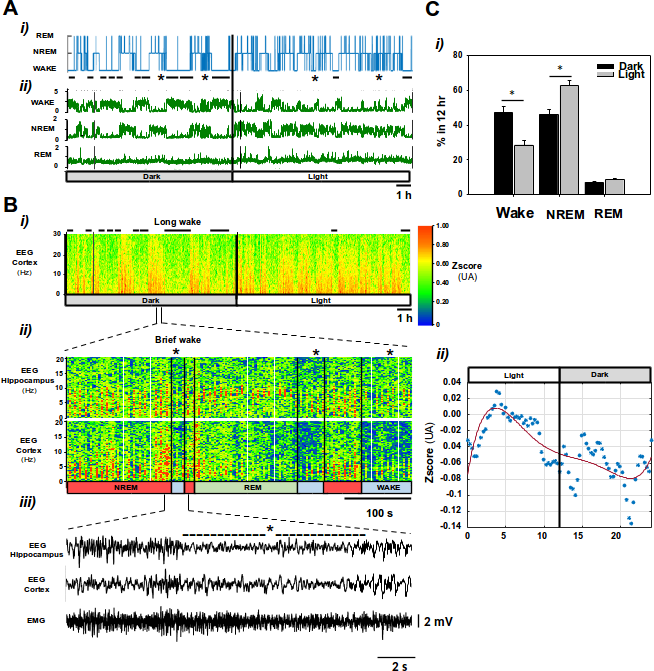
\includegraphics[width=\textwidth]{figuras_plos1.png}
	\caption{Representative data illustrating circadian modulation of sleep-wake behavior in C57Bl/6 mouse. A) Hypnogram (i) was generated by automatic sleep scoring of \WK/, \NREM/ and \REM/ sleep states (ii). Long (-) and brief (*) \WK/ bouts were observed, but only long \WK/ were affected along 12h/12h dark/light cycle. B) Long (-) and brief (*) \WK/ bouts were identified based on the frequency pattern of cortex and hippocampal EEG activity. }
          \label{fig_raw}
\end{figure}

\begin{figure}
	\vspace{1.0cm}
\begin{center} 
	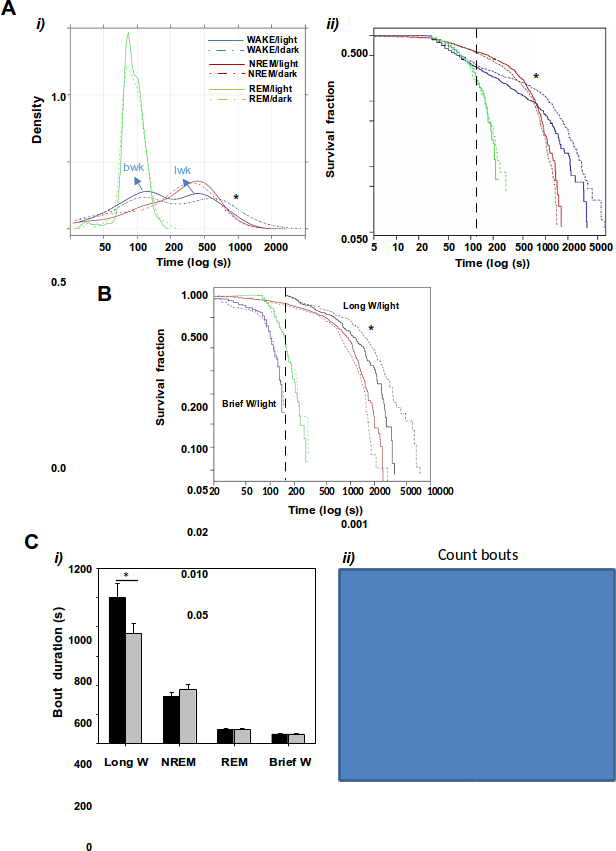
\includegraphics[height=16cm]{figuras_plos2.png}
	\caption{Statistics of \WK/, \NREM/ and \REM/ bout duration as a function of dark/light periods. A) Total amount of \WK/ and \NREM/ duration increased and decreased respectively during dark in comparison with light phase. B) Bouts duration histogram showed a clear bimodal density distribution of wake (brief- and long-\WK/) and probably also for \NREM/ epochs, while \REM/ distribution was unimodal; only the density of long-\WK/ varied during circadian rhythm, lasting longer in the dark (active) than light (inactive) phase. C) Cumulative \WK/ showed by Kaplan-Meyer survival curves exhibited a biexponential distribution (\WKB// and \WKL/, vertical bar) with a significant increment of \WKL/ duration in dark phase (*, Anova  $p <0.05$). }
	\label{fig_markov}
\end{center} 
\end{figure}

\begin{figure}
	\vspace{1.0cm}
\begin{center} 
	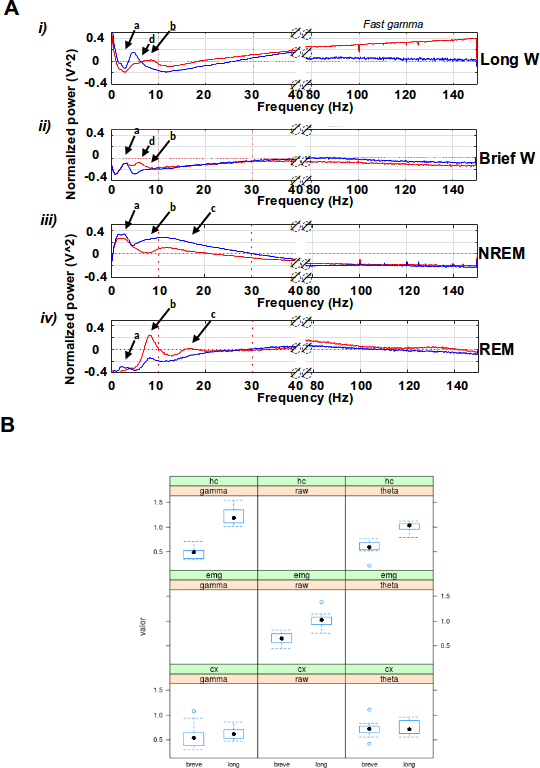
\includegraphics[ height=16 cm]{figuras_plos3b.png}\\
	\vspace{1.0cm}
	\caption{A. Spectral analysis of 24-hour sleep, during the 4 stages of sleep. Frontal cortex (Blue), hippocampus (Red). i) y ii) The hippocampal spectral content of the two substates of wake is different: long wake epochs had an augmented theta band with a characteristic 8 Hz peak, whereas in the brief wake a low frequency theta activity is observed at  6 Hz (arrow d). In addition, the fast gamma hippocampal frequencies of long wake epochs are significantly increased compared to brief wake. iii) During NREM sleep a predominance of delta and beta power, and a reduction of gamma band  are observed (arrows a and c respectively). iv) In REM there is a predominance of theta (arrow b) with delta and beta slow, and an increased gamma band with respect to NREM. B. EMG tone, hippocampal fast gamma and theta power are increased in long wake.}
	\label{fig_eeg}
\end{center} 
\end{figure}




\begin{figure}
	\vspace{1cm}
	TABLE 1. Probability of transitions between states and to remain in a state for discrete time steps
of 5 seconds applying a four-state Markov model to fit the mouse sleep-wake dynamics along 12/12
h dark/light cycle
\begin{center}
	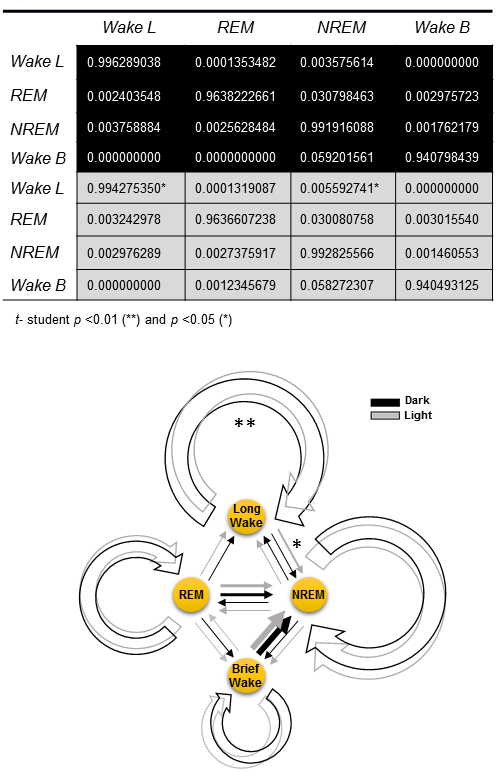
\includegraphics[height=16cm]{fmk_3.png}
\end{center}
	\caption{Diagram of four-state Markov model accounting for the \WK/-sleep dynamics across dark/light cycle. Circular arrows correspond to the probability of maintaining a state (i.e., the time spent in the corresponding state or bout duration), and straight arrows to transitions between states; arrows thickness are proportional to the corresponding probabilities (from Table 1), and the dark and light periods are represented in black and grey. The sleep-wake model of four states comprises of two \WK/ states (with spectral differences, see text): a long-\WK/ (\WKL/) and a brief-\WK/ (\WKB/); and of \NREM/ and \REM/ sleep states. States of \WKL/ and \NREM/ were more stable than \REM/ and \WKB/, while state transitions \WKB/ to \NREM/ and \REM/ to \NREM/ were the most probable. Circadian modulation increased the stability of \WKL/ mainly by reducing the transitions from \WKL/ to \NREM/ during dark active period (*, $ p  < 0.05$; and **,  $p  < 0.01$). }
          \label{fig_model}
\end{figure}

\end{document}

